\section{Evaluation}
\label{sec:evaluation}

% ~1.25 pages. Everything here is from report-v1.md (header, "Choosing the judge", "For writing the report") and
% eval/studies/report-v1.toml. Say early: one round, one code version, comparisons named before the runs.

\subsection{Benchmarks}
% Main suite: 48 requests (simple 5, medium 17, hard 13, proposal 8, casual 5); 42 should be built, 3 declined,
% 3 either. Each with an expected bounding box has a hand-written reference solution that builds at that size
% (eval/references.py), never shown to the model. None copied from the example library.
% Organic suite: 30 objects (animals, figures, ...), no expected size; no organic subject in the SDF examples.
% Appendix A lists every case.

The total benchmark was derived of 78 requests to the agent.
Form these 78 requests, 48 were mechanical parts and 30 were organic.
Each of the mechanical requests belonged to one of four categories: simple requests (5), medium-difficulty requests (17), hard-difficulty requests (13), and casual requests (13).
Casual requests are ones that do not follow a specific mechanical request, similar to organic style requests.
Each object in the casual was hand-checked as to whether the model should reject building the part, require building it, or allow either a rejection or build.

The organic suite is similar to the casual requests, except specifically focused on sculpting shapes.
For example, the 12th organic benchmark requests: "A turtle 60 mm long: a domed shell, four stubby legs, a head poking out the front and a short tail."

\subsection{Builders and configurations}
% Table 1: builders. Columns: model, where it runs (API / Google API / local RTX 3080), configs run.
%   claude-sonnet-5-5, claude-haiku-5-5, gemini-3.5-flash-lite, gemma-4-31b-it (Google API), gemma4:12b (local
%   default), qwen3.5:4b (local base), cad-qwen3.5:4b-v2 (fine-tuned), plus Thingiverse (organic only).
% Configs: rag-size (3 retrieved examples, measured-size message: the app's setup), norag-size (no examples),
% sdf (organic, 11 SDF examples), thingiverse-check (first matching download). 4 attempts max. 3 runs per pair.
% Gemma 31B, Haiku and the no-RAG Qwen arms were added during the round ("Changes during the round").
\TODO{text for Table 1}

% Table 1: from the round's rows (eval/results/studies/report-v1/, one arm per model, suite and config):
% 144 runs per main-suite arm (48 cases x 3), 90 per organic SDF arm (30 x 3), 30 Thingiverse runs; 2,118 in all.
\begin{table}[t]
  \centering
  \small
  \setlength{\tabcolsep}{3pt}
  \begin{tabular}{@{}llccc@{}}
    \toprule
    & & \multicolumn{2}{c}{Main suite} & Organic \\
    \cmidrule(lr){3-4} \cmidrule(l){5-5}
    Builder & Runs on & RAG & no RAG & SDF \\
    \midrule
    Claude Sonnet 5.5          & Anthropic     & \checkmark & \checkmark &            \\
    Claude Haiku 5.5           & Anthropic     & \checkmark & \checkmark & \checkmark \\
    Gemini 3.5 Flash Lite      & Google        & \checkmark & \checkmark & \checkmark \\
    Gemma 4 31B                & Google        & \checkmark &            &            \\
    Gemma 4 12B$^\dagger$      & local         & \checkmark &            &            \\
    Qwen3.5 4B fine-tuned      & local         & \checkmark & \checkmark & \checkmark \\
    Qwen3.5 4B (base)          & local         & \checkmark & \checkmark & \checkmark \\
    \midrule
    Thingiverse                & Thingiverse   & \multicolumn{2}{c}{--} & download \\
    \bottomrule
  \end{tabular}
  \caption{Builders and the configurations each was run with. \emph{RAG}: three retrieved examples in the prompt
    (the app's setup); \emph{no RAG}: none; \emph{SDF}: organic objects sculpted with SDF code and 11 SDF examples; Thingiverse
    search takes the first matching download instead. API models run on the provider's servers. Every model run allows up to 4 attempts and
    is repeated 3 times per case (Thingiverse once); 2,118 runs in all. Local models run in Ollama on one RTX 3080 (10\,GB). $^\dagger$The app's default local model.}
  \label{tab:builders}
\end{table}

\subsection{Metrics}
% Correct: built at the expected size (or declined when it should be); organic: a valid mesh.
% Right size + shape: correct and the visual judge passes it (organic: any part that came out and passes).
% Also: first-try rate, correct after k attempts, pass@k over the 3 repeats~\cite{chen2021codex},
% tokens, $ per correct part, time.
\TODO{metrics}

\subsection{Visual judge}
\label{sec:judge}
% Six views per part (front, right, top, bottom flat; two isometric), one request with the request text and the
% measured size; score 0-1 on four bands (match / minor / feature wrong / different object; top two pass).
% Choice: 4 judges x 204 items x 3 runs; items = 58 reference checks + 146 hand-graded parts (100 graded blind:
% no builder, config or judge score shown). Rule written before the runs: best held-out accuracy, the cheaper one
% if the interval overlaps the old judge's. It picks Sonnet; Sonnet for every part (~$5.90) was over the remaining
% budget, so gemini-3.8-flash (statistically tied, 92% vs 96%, p = 0.08) judges the main suite and Sonnet the
% organic suite, where gemini-3.8-flash is weak (71% vs 91%). State this deviation plainly. Results in Sec. 5.7.
\TODO{judge}

% Figure: renders copied by `pixi run -e cap6938 python -m scripts.report_figures judge-example`, which also prints
% the judge's replies quoted below (gemini-3.8-flash, report-v1, same verdict in all 3 runs).
\begin{figure*}[t]
  \centering
  \small
  \textit{``Can you make me something to stand my AA batteries up in? 8 of them in two rows of four, holes 15mm wide
    and 20mm deep, in an 80 x 40 x 25 block.''}\\[4pt]
  \begin{minipage}[t]{0.485\linewidth}
    \centering
    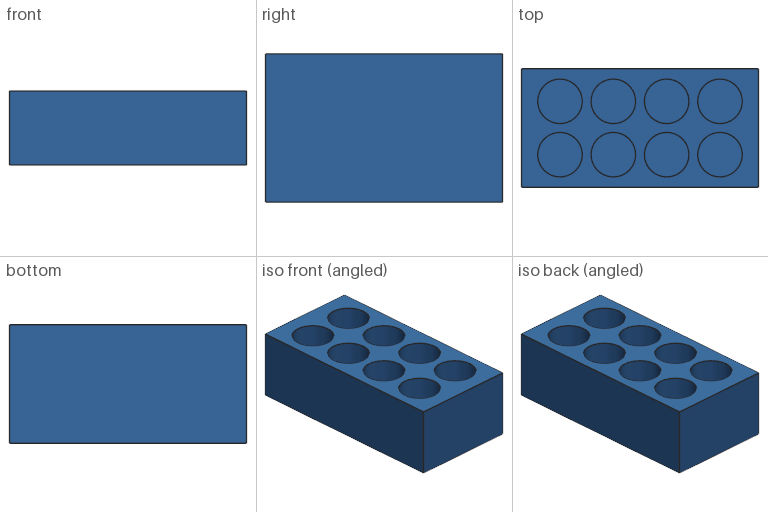
\includegraphics[width=\linewidth]{figures/judge_c01_reference.png}\\[2pt]
    (a) Reference solution: score 1.0 (\emph{pass}).
  \end{minipage}\hfill
  \begin{minipage}[t]{0.485\linewidth}
    \centering
    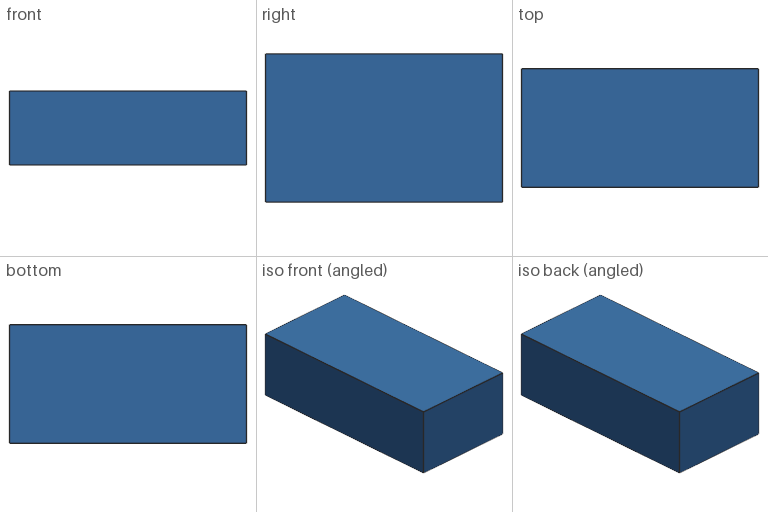
\includegraphics[width=\linewidth]{figures/judge_c01_gemma31b.png}\\[2pt]
    (b) Gemma 4 31B build: score 0.11 (\emph{fail}). ``Missing all 8 holes for the AA batteries; part is a
    completely solid block.''
  \end{minipage}
  \caption{What the visual judge sees: six views of the part (four flat, two angled), sent in one request with the
    request text and the measured size. Both parts measure $80 \times 40 \times 25$\,mm, so the size check accepts
    both; only the top and angled views show that (b) has no holes. The judge scores 1--10 on four bands (match,
    small deviations, a feature wrong, a different object), rescaled to 0--1; 0.5 and above passes. It gave each part
    the same score in all 3 runs, and the hand grade for (b) is ``different object''.}
  \label{fig:judge}
\end{figure*}

% Figure: made by `pixi run -e cap6938 python -m scripts.report_figures render-fix`. From development, before the
% report round: judge gemini-3.1-flash-lite, render/prompt v1 vs v2 (eval/results/judge-gemini-3.1-flash-lite.md).
\begin{figure}[t]
  \centering
  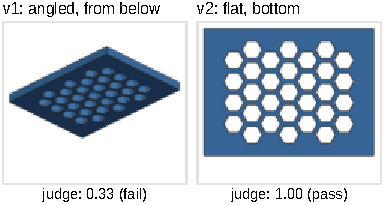
\includegraphics[width=\linewidth]{figures/render_fix.pdf}
  \caption{Why the renders include a flat bottom view. The reference solution for a honeycomb panel with hexagonal
    through-holes, seen from below in our first render version (left) and the current one (right). From the angled
    view the first judge, gemini-3.1-flash-lite, concluded ``the holes are not actual through-holes; they are
    recessed pockets'' and failed this correct part, although the flat top view already showed the background
    through the holes. With the flat bottom view, and a prompt line saying that only flat views show a through-hole as
    see-through, it passed. Fig.~\ref{fig:failures}b shows the reverse case: pockets that the flat bottom view exposes.}
  \label{fig:render-fix}
\end{figure}

\subsection{Statistics}
% Rate = mean over cases of each case's rate over 3 runs. 95% intervals: bootstrap over cases~\cite{efron1993bootstrap}
% (repeats are not independent). Comparisons paired by case: mean difference with interval and exact sign test.
% Judges: McNemar's exact test~\cite{mcnemar1947}, Cohen's kappa~\cite{cohen1960kappa}. Code: eval/stats.py.
% The compared pairs were written in the manifest before the runs.
\TODO{statistics}
